\addtocontents{toc}{\protect\setcounter{tocdepth}{0}}
\section{Anexo}

\begin{frame}{Inicializaci\'on de Par\'ametros en ACO (OE 1)}
    \begin{columns}
        \hspace{-1cm}
        \begin{column}{0.4\textwidth}
            \begin{enumerate}[A)] \fontsize{10pt}{5}\selectfont
                \item Umbrales $\theta$ y $Max\_Angle$ 
                \begin{enumerate}[1]\fontsize{10pt}{5}\selectfont
                    \item $[0, \theta]$
                    \item $]\theta, Max\_Angle]$
                    \item $ > Max\_Angle$
                \end{enumerate}
                % \begin{itemize} \fontsize{10pt}{5}\selectfont
                %     \item $max(2.5 \theta, 90\degree)$
                %     \item $\measuredangle (e_{i}, e_{j})> Max\_Angle$
                % \end{itemize}
                \item Factor {\it Max\_Axial\_Displacement}: Curvatura y Magnitud entre segmentos
                %\item {\it Max\_Score}
                %\item Valor Inicial $\tau_0$
                \item Criterio de finalizaci\'on de un recorrido
            \end{enumerate}
        \end{column}
        \begin{column}{0.25\textwidth}
            \centering
            \begin{figure}
                %\centering
                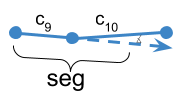
\includegraphics[scale=0.55]{Pictures/ant-params-1.png}
                \caption{Caso A1}
            \end{figure}
            \vspace{0.1cm}
            \begin{figure}
                %\centering
                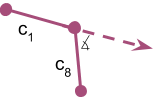
\includegraphics[scale=0.55]{Pictures/ant-params-2.png}
                \caption{Caso A2}
            \end{figure}
        \end{column}
        \begin{column}{0.25\textwidth}
            \begin{figure}
                 \centering
                 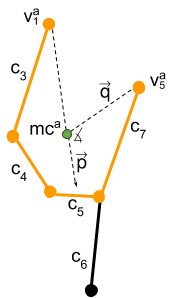
\includegraphics[scale=0.55]{Pictures/ant-params-3.png}
                 \caption{Caso B}
             \end{figure}
        \end{column}
    \end{columns}
\end{frame}

\note[itemize]{
    \item Es necesario definir inicialmente 2 umbrales, el umbral teta y el umbral max angle. Estos umbrales nos definen 3 rangos. En estos rangos se clasifica el \'angulo que forman 2 aristas entre s\'i. Si el \'angulo pertenece al primer rango, se sabe con certeza que ambas aristas pertenecen al mismo filamento. As\'i, estas 2 aristas pertenecen al mismo trozo o segmento de filamento, definido como seg.
    
    
    Por otra parte, si este \'angulo es mayor que el umbra Max Angle, se tiene certeza que ambas aristas no pertenecen al mismo filamento. 
    \item Dado que al utilizar un grafo que no considera la curvatura en el c\'alculo de \'angulos, es posible perder informaci\'on, por lo que los filamentos que tengan aristas cuyos \'angulos pertenezcan al segundo 2do rango , necesitan de an\'alis adicional para determinar si se descartan o no.
    
    
    \item Otro elemento a considerar es el Factor Max Axial Displacement, el que es utilizado para otorgar flexibilidad a la evaluaci\'on adicional mencionada previamente, influyendo en la evaliaci\'on de la curvatura de un filamento, as\'i como en la magnitud entre segmentos1

}

\begin{frame}{Heur\'istica Miope}
    \begin{equation}%\fontsize{9pt}{7.2}\selectfont
    \eta_{ij} = 
        \begin{cases} 
        \text{Max\_Score si } \measuredangle(c_{ij}, s_{n}^{P}) \in [0, \theta],\\[3ex]
        
        \text{Max\_Score} \cdot \left(1 - \dfrac{ \left| \measuredangle(c_{ij}, s_{n}^{P}) - \frac{\theta}{2} \right|} {180} \right)  \text{ si } \measuredangle(c_{ij}, s_{n}^{P}) \in \quad ]\theta, \text{Max\_Angle}],\\[3ex]
        
        \text{0 en otro caso.}
        \end{cases}
    \end{equation}    
\end{frame}

\note[itemize]{
  \item En particular, la heur\'istica miope $\eta_{ij}$ entrega una puntuaci\'on que disminuye a medida que el \'angulo mencionado aumenta, siendo el rango $[0, \theta]$ el que otorga la puntuaci\'on m\'axima de $Max\_Score$. Si el \'angulo es mayor a $Max\_Angle$ la puntuaci\'on corresponde a 0. Para el rango intermedio $]\theta, Max\_Angle]$, la puntuaci\'on depende de la diferencia entre el \'angulo formando entre la arista $c_{ij} \in N(s^{P})$ y $s_{n}^{P}$. Mientras m\'as aumenta esta diferencia, menor es la puntuaci\'on asignada.
}

\begin{frame}{Extensi\'on de Anti-feromonas sobre un segmento (OE 1)}
    \centering
    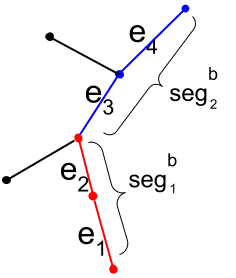
\includegraphics[scale=0.4]{Pictures/ant_segments_simple_case.png}
    \begin{itemize}
        \item Cada arista del segmento forma un \'angulo en el rango $[0, \theta]$ con sus vecinos
        \item Penalizaci\'on de $e_3$ se asocia al $seg^{b}_{1}$, sin perjudicar otros caminos que pasen por $e_3$ pero no por el segmento $seg^{b}_{1}$.
    \end{itemize}
\end{frame}

\note[itemize]{
  \item En este ejemplo se observa el camino de una hormiga $b$ compuesto por 2 segmentos. El \'angulo entre las aristas e1 y e2, as\'i como el \'angulo de e3 con e4 pertenece al rango 0, theta.
  \item El \'angulo entre las aristas $e_2$ y $e_3$ pertenece al rango $]\theta, Max\_Angle]$, lo que determina el fin del segmento $seg^{b}_1$ e inicia el segmento $seg^{b}_2$.
}

\begin{frame}{Curvatura de una soluci\'on y Magnitud de desplazamiento entre segmentos}
    \centering
    \begin{equation}\fontsize{9pt}{7.2}\selectfont
    \tau_{ij} \leftarrow
        \begin{cases}
        \tau_{ij} \cdot \gamma \text{ si } \measuredangle(proy(\Vec{p}), \Vec{q}) \geq \theta \cdot \text{Max\_Axial\_Displacement},\\[3ex]
        
        \text{0 si } \tau_{ij} \leq 0.25, \\[3ex]
        \tau_{ij} \quad \text{en otro caso.}
        \end{cases}
    \end{equation}
    \vspace{1cm}
    \begin{equation}\fontsize{9pt}{7.2}\selectfont
    \tau_{ij} \leftarrow
        \begin{cases}
        \begin{split}
         \tau_{ij} \cdot \gamma \text{ si } & \sin(\measuredangle seg^{a}_{pMaxMin}) > seg^{a}_{iMax} \cdot 0.1 \cdot \text{Max\_Axial\_Displacement} \\ & \land \measuredangle seg^{a}_{pMaxMin}) > \theta,
        \end{split}
        \\[3ex]
        
        \text{0 si } \tau_{ij} \leq 0.25, \\[3ex]
        \tau_{ij} \quad \text{en otro caso}.
        \end{cases}
\end{equation}
\end{frame}

\note[itemize]{

  \item El \'angulo entre la proyecci\'on de $\Vec{p}$ y $\Vec{q}$ no debe superar el valor que resulta al multiplicar el \'angulo $\theta$ por el factor {\it Max\_Axial\_Displacement}. Este factor permite flexibilizar la tolerancia de la curvatura en base a $\theta$. Si el recorrido de la hormiga tiene un \'angulo igual o mayor al umbral, implica que la soluci\'on encontrada es demasiado curva para representar un filamento, por lo que es penalizada y descartada. 
  

  \item Para la magnitud de desplazamiento entre segmentos se define el segmento m\'as largo entre ambos segmentos comparados, en un camino $a$, como $seg^{a}_{iMax}$ , mientras que el segmento menor es $seg^{a}_{jMin}$. El \'angulo entre $seg^{a}_{jMin}$ y la proyecci\'on de $seg^{a}_{iMax}$ se define como 
$\measuredangle seg^{a}_{pMaxMin}$ por simplicidad. \bf{En el caso de que el \'angulo $\measuredangle seg^{a}_{pMaxMin}$ este en el rango $[0, \theta]$ se entiende que se respeta el criterio de m\'aximo desplazamiento.}
}

\begin{frame}{Ponderaci\'on de los par\'ametros (OE 3)}

    \begin{itemize}%\fontsize{9pt}{12}\selectfont
    \item No es posible utilizar un \'unico par\'ametro para obtener una ponderaci\'on directa
    \item Construcci\'on de soluciones: $\frac{100}{n}$\% el grado de los nodos, y el remanente para el \'angulo entre aristas, con $n$ como el n\'umero de aristas.
    \item M\'etodo de b\'usqueda no local: 100\% posici\'on de la arista.
    \item Actualizaci\'on de feromonas: 
    \begin{itemize}%\fontsize{9pt}{12}\selectfont
        \item Caso General: 50\% curvatura, 50\% diferencia de magnitud entre segmentos
        \item Neuronas: $33.\overline{3}\%$ curvatura, $33.\overline{3}\%$ diferencia de magnitud entre segmentos y $33.\overline{3}\%$ informaci\'on topol\'ogica de centralidad.
    \end{itemize}
\end{itemize}
\end{frame}

\begin{frame}{Par\'ametros del Algoritmo Propuesto (AP) (OE 3)}
    \centering
    \resizebox{\textwidth}{!}{
    %\centering
    \begin{tabular}{|c|c|c|c|c|}
        \hline
        & 
        & 
        \multirow{4}{1.5cm}{\it Max Axial Displ.} & \multirow{4}{1.5cm}{Permite Superposici\'on} &
        \multirow{4}{2cm}{Aplica Heur\'istica Asignaci\'on Completa}\\
        \diagbox[width=10em]{C\'elula}{Par\'ametro} & 
        $\theta$ & & &\\
        & & & &\\
         \hline
        Neurona (AP N) & 45\textdegree & 2 & Si & No\\
        MT Planta (AP MT-P) & 30\textdegree & 1.5 & Si & Si\\
        MT Animal (AP MT-A) & 60\textdegree & 2.5 & Si & Si\\
        Sint\'etico (AP S) & 45\textdegree & 1.5 & Si & No \\
        \hline
    \end{tabular}
}
\end{frame}

\begin{frame}{VI, \'Indice Rand e \'Indice Jaccard}
\resizebox{\textwidth}{!}{
    \begin{tabular}{|c|c|c|c|c|c|}
        \hline
        Figura & Config. de Par\'ametros & VI Max & VI & Rand & Jaccard \\ \hline
         4.1 & MT-P  & 2.3978 & 1.6360 & 0.7646 & 0.2485 \\
         4.1 & S1  & 2.3978 & 0.7091 & 0.8637 & 0.4750  \\
         4.2 & MT-P & 3.0445 & 2.2296 & 0.7276 & 0.1806 \\
         4.2 & S2 & 3.0445 & 2.5878 & 0.7276 & 0.1673  \\
         4.3 & MT-P & 3.4965 & 2.1656 & 0.8658 & 0.2407 \\
         4.4 & MT-P & 3.7612 & 2.6285 & 0.8683 & 0.2488  \\
         4.5 & MT-P & 1.9459 & 0.4286 & 0.8929 & 0.40 \\
         4.6 & N & 6.0258 & 1.7950 & 0.8864 & 0.1389 \\
         4.7 & N & 5.0814 & 3.7256 & 0.8775 & 0.0703 \\
         4.8 & N & 4.2046 & 1.0060 & 0.8794 & 0.2157 \\ \hline
    \end{tabular}
    %\caption{VI $\in [0, VI\_Max]$, Rand y Jaccard $\in [0, 1]$ }
}
\end{frame}



\begin{frame}{Implementaci\'on del Algoritmo Propuesto (OE 2)}
    \begin{itemize}
        \item Pre y post procesamiento de resultados en {\tt Python}: 
        \begin{itemize}
            \item Pre: Extracci\'on de un grafo (JSON), a partir de una imagen (PNG),  mediante {\tt sknw}/{\tt NetworkX}
            \item Post: Visualizaci\'on de resultados
        \end{itemize}
        
        \item Algoritmo Propuesto en {\tt C++}. Par\'ametros de entrada:
        \begin{itemize}
            \item Imagen a analizar (PNG) y el grafo (JSON)
            \item Tipo de c\'elula
            \item Color del fondo/segundo plano
            \item Opcionales: Nivel de debugging
        \end{itemize}
        
        
    \end{itemize}
\end{frame}

\begin{frame}{VI, \'Indice Rand e \'Indice Jaccard}
%    La mayor\'ia de los criterios para comparar particiones mediante conteo de pares   se basa en la 
    
    %suele fundamentarse en el uso de la matriz de confusi\'on, tambi\'en llamada matriz de asociaci\'on o tabla de contingencia \cite{meilua2007comparing}. Esta tabla considera 4 casos en los que puede estar un par de elementos del {\it data set}, que para el caso de la individualizaci\'on de filamentos son pares de aristas, en las particiones $C$ y $C'$:

    \begin{itemize}\fontsize{9pt}{10}\selectfont
        \item Mayor\'ia de los criterios para comparar particiones $\rightarrow$ matriz de confusi\'on/asociaci\'on o tabla de contingencia.
        \item $N_{11}$: N\'umero de pares que est\'an en el mismo cluster en $C$ y $C'$
        \item $N_{00}$: N\'umero de pares que est\'an en distintos clusters en $C$ y $C'$
        \item $N_{10}$: N\'umero de pares que est\'an en el mismo cluster en $C$ pero no en $C'$
        \item $N_{01}$: N\'umero de pares que est\'an en el mismo cluster en $C'$ pero no en $C$
        \item $N_{11} + N_{00} + N_{10} + N_{01} = \frac{n(n-1)}{2}$, con n como el n\'umero de aristas.
        \item Asociaci\'on de casos con evaluaciones de clasificaci\'on
    \end{itemize}

    %\resizebox{\textwidth}{!}{
    \makebox[\linewidth][c]{\fontsize{10pt}{12}\selectfont
        \begin{tabular}{|c|c|}
        \hline
            Casos para un par de aristas & Clasificaci\'on \\ \hline
            $N_{11}$ & Verdadero Positivo ({\it True Positive} o TP) \\
            $N_{00}$ & Verdadero Negativo ({\it True Negative} o TN)\\
            $N_{10}$ & Falso Positivo ({\it False Positive} o FP)\\
            $N_{01}$ & Falso Negativo ({\it False Negative} o FN)\\ \hline
        \end{tabular}
    }
\end{frame}

\begin{frame}{\'Indice Rand y Jaccard}
    \begin{equation}\fontsize{9pt}{7.2}\selectfont
        \mathcal{R}(C,C^{\prime}) = \frac{N_{11} + N_{00}}{n(n-1)/2} = \frac{TP + TN}{TP + TN + FP + FN}
    \end{equation}
    \vspace{0.2cm}
    \begin{equation}\fontsize{9pt}{7.2}\selectfont
        \mathcal{J}(C,C^{\prime}) = \frac{N_{11}}{N_{11} + N_{01} + N_{10}} = \frac{TP}{TP + FP + FN}
    \end{equation}
    \vspace{0.2cm}
    \begin{equation}\fontsize{9pt}{7.2}\selectfont
        \text{Precision} = \frac{TP}{TP + FP}
    \end{equation}
    \vspace{0.2cm}
    \begin{equation}\fontsize{9pt}{7.2}\selectfont
        \text{Recall} = \frac{TP}{TP + FN}
    \end{equation}
\end{frame}



% \begin{frame}{Ponderaci\'on de las caracter\'isticas}
%     \begin{itemize}\fontsize{9pt}{12}\selectfont
%     \item No es posible utilizar un \'unico par\'ametro para obtener una ponderaci\'on directa
%     %El uso de diversas caracter\'isticas en distintas partes del algoritmo propuesto
    
%     %Dado que las diversas caracter\'isticas utilizadas en el algoritmo propuesto se encuentran en distintos m\'etodos de la metaheur\'istica ACO, 
%     \item Construcci\'on de soluciones: $\frac{100}{n}$\% el grado de los nodos, y el remanente para el \'angulo entre aristas, con $n$ como el n\'umero de aristas.
%     \item M\'etodo de b\'usqueda no local: 100\% posici\'on de la arista.
%     \item Actualizaci\'on de feromonas: 50\% curvatura, 50\% diferencia de magnitud entre segmentos. En el caso espec\'ifico de las neuronas, corresponde a $33.\overline{3}\%$ curvatura, $33.\overline{3}\%$ diferencia de magnitud entre segmentos y $33.\overline{3}\%$ informaci\'on topol\'ogica de centralidad.
% \end{itemize}
% \end{frame}